\subsection{معیارهای ارزیابی}
\label{subsec:eval}
معیارهای ارزیابی را می‌توان به دسته‌ی کلی  معیارهای دسته بندی و رگرسیون تقسیم کرد.  معیارهای دسته بندی را می‌توان با استفاده از \واژه{ماتریس درهم‌ریختگی} محاسبه نمود. در ماتریس درهم ریختگی پیش‌بینی خطا، عناصر  به صورت زیر تعریف می‌شوند.  همچنین نحوه‌ی محاسبه‌ی معیارها در جدول \ref{tab:eval-metircs} آمده است. 
\begin{itemize}
	\setlength\itemsep{.01em}
\item \lr{TP} : 
تعداد داده‌های حاوی خطا که به درستی تشخیص داده شدند
\item \lr{FP}: 
تعداد داده‌های سالم که به عنوان خطادار پیش‌بینی شدند
\item \lr{TN}:
تعداد داده‌های سالم که به درستی تشخیص داده شدند
\item \lr{FN}: 
تعداد داده‌های حاوی خطا که به عنوان داده‌ی سالم پیش‌بینی شدند

\end{itemize}


\begin{table}[H] 
		\renewcommand*{\arraystretch}{1.5}	
	\centering \caption{فرمول‌های محاسبه‌ی معیارهای ارزیابی}
	\label{tab:eval-metircs}
	\newcolumntype{C}{>{\centering\arraybackslash} m } 

	\begin{tabular}{|C{1.5cm} |C{2cm}|C{4.5cm}|C{6cm} |}
 
	\hline
	\hline
	نام معیار & نام لاتین & نحوه‌ی محاسبه & توضیح
		\\
	\hline
	\hline
	نرخ مثبت کاذب &
	\lr{False Positive Rate (PF)}  &
	$ \displaystyle \frac{FP}{TN+FP} $ &
	نسبت تعداد داده‌هایی که به اشتباه خطادار پیش‌بینی شده‌اند به تعداد کل داده‌های بدون خطا
	\\
	\hline
	صحت & 
		\lr{Accuracy} & $ \displaystyle \frac{TP+TN}{TP+FP+TN+FN}$ &
	نسبت	تعداد پیش‌بینی‌های درست به تعداد کل پیش‌بینی‌ها
		
	\\
	\hline
	دقت &
	\lr{Precision} & $\displaystyle \frac{TP}{TP+FP}$ &
نسبت تعداد داده‌هایی که به درستی خطادار پیش‌بینی شده‌اند به تعداد کل داده‌هایی که خطادار پیش‌بینی شده‌اند
	\\
	\hline
	بازخوانی & 
	\lr{Recall (PD)} & $\displaystyle \frac{TP}{TP+FN}$ &
	نسبت تعداد داده‌هایی که به درستی خطادار پیش‌بینی شده‌اند به تعداد کل داده‌های خطادار
	\\
	\hline
	معیار اف &
	\lr{F-Measure} & $ \displaystyle \frac{2 \times Precision \times Recall}{Precision + Recall}$ &
	از آنجا که در بین معیارهای دقت و بازخوانی مصالحه وجود دارد معیار اف ترکیبی از آن دو را در نظر می‌گیرد
	\\
	\hline
	\end{tabular}
\end{table}

دو معیار دیگر نیز که در پژوهش‌ها کاربرد دارند عبارتند از 
\lr{AUC }\LTRfootnote{Area under curve}  و 
\lr{AUCEC }\LTRfootnote{Area under cost-effectiveness curve }
که هر دو به مساحت زیر یک منحنی اشاره می‌کنند. \lr{AUC}  مساحت زیر نمودار
\lr{ROC }\LTRfootnote{Reciever operating characteristic}  
را اندازه‌گیری می‌کند. در نمودار \lr{ROC}،  محورهای عمودی و افقی را به ترتیب بازخوانی و  نرخ مثبت کاذب تشکیل می‌دهد.  با تغییر آستانه پیش‌بینی برای یک مدل می‌توان میزان بازخوانی و  نرخ مثبت کاذب را تغییر داده و بدین ترتیب منحنی \lr{ROC} را رسم نمود. یک مدل بی‌نقص دارای مساحت زیر نمودار 1 است. برای یک مدل تصادفی  منحنی از مبدا به نقطه‌ی (1\lr{,}1) رسم خواهد شد. یک نمونه از منحنی \lr{ROC} در شکل \ref{fig:ROC} آمده است. \\

\begin{figure}
	\centering
	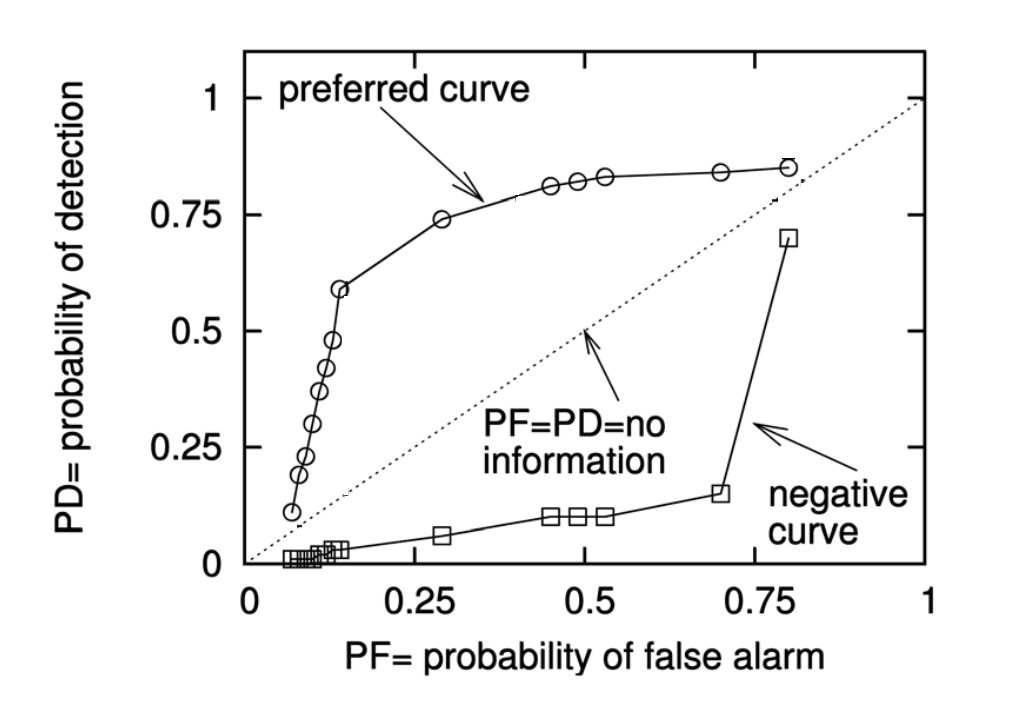
\includegraphics[width=.60\textwidth]{img/ROC.PNG}
	\caption{ نمونه‌ای از نمودار \lr{ROC} \cite{menzies2007data}}
	\label{fig:ROC}
\end{figure}

معیار \lr{AUCEC} معیاری است که تعداد خطوطی از برنامه که  توسط تیم تضمین کیفیت و یا توسعه دهندگان نیاز است بررسی و آزموده شود را در نظر می‌گیرد. ایده‌ی  موثر بودن از نظر هزینه\LTRfootnote{Cost-effectiveness}
برای مدل‌های ‌‌ خطا برای اولین بار توسط آریشلم و همکاران \cite{arisholm2007data} ارائه گردید. موثر بودن از نظر هزینه به این معنا است که چه تعداد خطا با بررسی و یا تست  \lr{$\%n$ } اول خطوط می‌توان یافت. به عبارت دیگر اگر یک مدل پیش‌بینی خطا بتواند تعداد خطای بیشتری را با بررسی و تلاش در آزمون کمتر، نسبت به باقی مدل‌ها بیابد می‌توان گفت که تاثیر آن از نظر هزینه بیشتر است. دو منحنی در  قسمت راست شکل \ref{fig:AUCEC} برای دو مدل پیش‌بینی مختلف آمده است. هر دو مدل دارای سطح زیر نمودار یکسانی هستند اما زمانی که 20\lr{\%}  اول محور افقی در نظر گرفته می‌شود مدل 
\lr{P$_2$}
  کارایی بهتری دارد. نمودار سمت چپ مدل‌های تصادفی، عملی\LTRfootnote {Practical} و بهینه را نشان می‌دهد.

\begin{figure}[H]
	\centering
	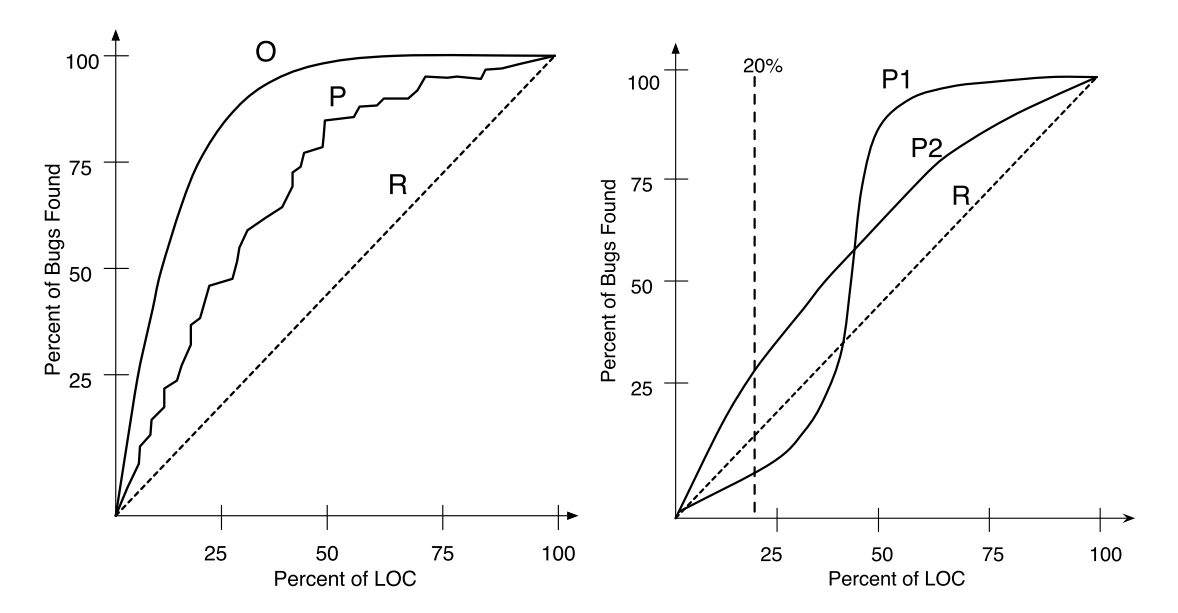
\includegraphics[width=.7\textwidth]{img/AUCEC.PNG}
	\begin{tabular}{c c c}
		\lr{O = optimal} & \lr{P = practical} &  \lr{R = random}\\
	 
	\end{tabular}
	\caption{ نمودار موثر بودن از نظر هزینه \cite{rahman2011bugcache}}
	\label{fig:AUCEC}
\end{figure}

معیارهایی که برای ارزیابی نتایج حاصل از روش رگرسیون به کار گرفته می‌شوند بر اساس همبستگی\LTRfootnote{Correlation} میان تعداد خطاهای پیش‌بینی شده و خطاهای واقعی محاسبه می‌شوند. نماینده‌ی این معیارها را می‌توان همبستگی اسپیرمن، پیرسون و $ R^2$ دانست \cite{nam2014survey}. 